\documentclass{article}
\usepackage[utf8]{inputenc}
\usepackage{miller,siunitx,subcaption,float,newfloat,amsmath,amssymb,chemformula,graphicx}
\usepackage[labelfont=bf]{caption}
\usepackage{xr} % necessary for external references
\usepackage{lineno}
\linenumbers
%%%%%%%%%%%%%%%%%%%%%%%%%%%%
% This section is part of where the magic happens
%%%%%%%%%%%%%%%%%%%%%%%%%%%%
\makeatletter
\newcommand*{\addFileDependency}[1]{% argument=file name and extension
  \typeout{(#1)}
  \@addtofilelist{#1}
  \IfFileExists{#1}{}{\typeout{No file #1.}}
}
\makeatother

\newcommand*{\myexternaldocument}[1]{%
    \externaldocument{#1}%
    \addFileDependency{#1.tex}%
    \addFileDependency{#1.aux}%
}

\myexternaldocument{main_supporting}

\begin{document}
    \section{Abstract}
This document will highlight several features of LaTeX that allow for compilation of multiple documents within the same directory.
While these methods are powerful, unfortunately they sometimes run afoul of Overleaf's compilation paradigm, and file management, so some troubleshooting may be necessary.
    \section{Introduction}
This project contains 4 compilable documents, several of which are interconnected.
This is made possible by the package \verb|xr| and the addition of the \verb|latexmkrc| file.

The basic idea is that we can tell LaTeX that we want to compile a given file \textit{before} another file, and then use the results of the compilation in our new file.
We have 3 main connected files, the supporting information, the main article, and the response to reviewers.
In general, we want the compilation order to be:
\begin{center}
    Supporting Info $\to$ Main Article $\to$ Response to Reviewers
\end{center}
This ensures that any references to the supporting information in the main text are compiled before the main text, and any references to the main text from the reviewer response are compiled first.

The first thing to note is that the compilation target can be set by the user within the Overleaf main menu:
\begin{center}
    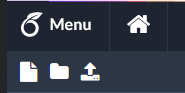
\includegraphics[width=0.3\textwidth,keepaspectratio]{tutorial/OverleafMenu.png} $\to$
    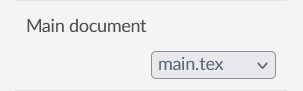
\includegraphics[width=0.3\textwidth,keepaspectratio]{tutorial/MainDoc.png}
\end{center}
This allows you to work on any of these individual documents separately, however be aware that the compile time may increase significantly when working on a document with many dependencies (such as the response to reviewers).
\subsection{Troubleshooting}
Sometimes, Overleaf seems to display the pdf that matches the name of the file that is currently selected, so changes in compilation may not be reflected if the wrong .tex file is selected.
Try selecting the .tex file of the pdf you want to view, and it may sort itself out.

If the above does not work, sometimes it is necessary to view or clear the cached files.
All of the compiled files can be viewed in the ``Other logs and files'' dialog, and the compiled files can be cleared using the ``Clear cached files'' dialog:
\begin{center}
    
\includegraphics[width=0.3\textwidth,keepaspectratio]{tutorial/CachedFiles.png}
\end{center}
Both of these dialogs are at the very bottom of the ``logs'' pane which is immediately adjacent to the ``Compile''/``Recompile'' button.
    \section{Results and Discussion}
Let's now demonstrate some of this functionality.
%
    \subsection{Figure Referencing}
%
With the compilation of the supporting information happening first, and the definition of a special supporting figure environment, we can very easily reference these figures in our main text.
Supporting Figure S\ref{sfig:example}.
We can also reference subfigures in our supporting figures.
Supporting Figure S\ref{sfig:sub-example1}.

We can also put some subfigures in our main text to be referenced in our response to reviewers:
\begin{figure}[H]
    \centering
    \begin{subfigure}{0.45\textwidth}
        \centering
        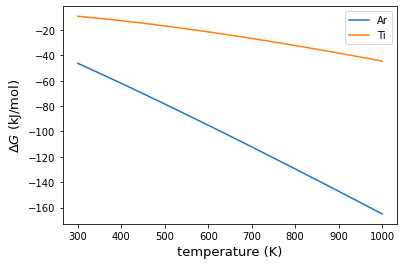
\includegraphics[width=\textwidth,keepaspectratio]{figures/DeltaG.png}
        \caption{}
        \label{fig:example1}
    \end{subfigure}
    \begin{subfigure}{0.45\textwidth}
        \centering
        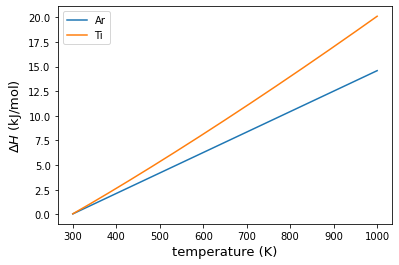
\includegraphics[width=\textwidth,keepaspectratio]{figures/DeltaH.png}
        \caption{}
        \label{fig:example2}
    \end{subfigure}
    \caption{
    (\subref{fig:example1}) basic demonstration of the subref command for a subfigure.
    (\subref{fig:example2}) The other subfigure
    }
    \label{fig:example-main}
\end{figure}
The subref command allows you to extract just the alphabetical label for the figure, while the ref command will extract the full reference.
For example, Figure \ref{fig:example1} (ref) or Figure part \subref{fig:example1} (subref).
This only works if the correct labels are attached.
%
    \subsection{Line and Page Numbers}
%
Line and page numbers are extremely useful when responding to reviewers.
As such, it's quite convenient to be able to label and reference changes between the two documents.
This line contains a label,\label{point:1} and a linelabel,\linelabel{line:1} which will allow me to reference it in the response to reviewers.
%
    \subsection{Word Counts}
%
Word counts can be done with great accuracy using \verb|texcount| which is a command line tool installed with most LaTeX distributions.
It is possible to count multiple files at once, and it provides detailed statistics.
\begin{center}
    \verb|texcount 1_introduction.tex 2_results.tex|
\end{center}
%
    \subsection{Track Changes}
%
It is possible to obtain a ``marked up'' version of your manuscript by using the command line tool \verb|latexdiff|.
This tool takes two .tex files as inputs, and outputs a .tex file which will compile to an annotated track changes version.
\begin{center}
    \verb|latexdiff oldfile.tex currentfile.tex > markup.tex|
\end{center}
    \section{Materials and Methods}
    \section{Conclusions}
\end{document}
